\chapter{Literature Review}\label{chapter:literature_review}

\section{Actor Programming Model}
Actor programming model is a programming paradigm designed for concurrent computation. The concept of an actor was originally introduced by Carl Hewitt\cite{hewitt} and he along with Agha\cite{agha} have been involved in development of both the actor theory as well as its implementation. An actor is a fundamental unit of computation. It is neither an operating system process nor a thread, but a lightweight process. It has to embody three essential things:
\begin{itemize}
  \item Processing
  \item Storage
  \item Communication
\end{itemize}
Actors have addresses, each actor can have multiple addresses or multiple addresses can belong to one actor. Actors communicate with each other in a non-blocking way by message passing, thus removing the need of explicit locks. An actor can send message to actors in another system or it can also send message to itself for recursion. An actor can send messages only to addresses that it receives in the message, addresses that it already had before it received the message or addresses of actors that it creates while processing the message. Each actor has a mailbox. A mailbox is a queue of messages that have been sent by other actors or processes and not yet consumed, where mailbox is also an actor. The order in which the messages are delivered is non-deterministic.
When an actor receives a message it can:
(Essentially, an actor is a computational agent which carries out its actions in response to accepting a communication. The actions it may carry out are:)~\parencite{hewitt}
\begin{itemize}
  \item Create other actors
  \item Send messages to itself, other known actors or reply to actor who sent the message
  \item Designate how it is going to handle next message, i.e. Specify replacement behavior
\end{itemize}


There are three ways in which an actor A, upon accepting a communication K, can know of a target to which it can send a communication. These are:~\parencite{agha}
\begin{itemize}
  \item the target was known to the actor a before it accepted the communication
  \item the target became known when the message was accepted because it was contained in the message or
  \item the target is the mail address of a new actor created as a result of accepting the message
\end{itemize}

Actors do not have shared mutable state. All mutable state is private to the actor and all shared state is immutable
Actor communicate with each other asynchronous message passing which is immutable.
Each actor processes only one message at a time, and unless it is a broadcast message, a message is not processed two times.

An actor alone does nothing much, they must come in a system. An actor system is a group of actors working together in certain hierarchy.
In the actor model, concurrency is inherent because of the way it is designed. Also, there is no guarantee that the message sent to an actor will arrive sequentially.

\subsection{Error Handling in Actor Model}

Error handling in actor model is based on "let it crash" philosophy. The isolated, shared nothing trait of actors allows a single actor to fail without affecting any other actors. Furthermore, the actor model itself can be used for fault tolerance, by spawning hierarchy trees of actors for supervision. Once an actor crashes, the supervising actor receives a messages and can react. A supervisor usually handles the error in actors by restarting the actor, stopping the actor, ignoring the error or escalating the error to its own supervisor. \url{http://berb.github.io/diploma-thesis/original/054_actors.html}

Several programming languages like Act 1, 2 and 3, Acttalk etc were created when actor system was newly introduced by Hewitt and Agha.

\subsection{Differences From Conventional Programming Languages}
In traditional programming languages, the control flow of a concurrent program is divided over a number of threads. Each thread operates concurrently and control can switch from one thread to another non-deterministically. If two threads have access to the same data (objects), they might cause erroneous behavior (so-called race conditions) because of this non-determinacy. Therefore, thread-based programming languages introduce locks (in the form of monitors, semaphores, ...) which enable the construction of so-called critical sections, which are pieces of program code in which only one thread can run sequentially at a time.

The advantages of the thread-based model are that the model itself is easy to understand, it is efficiently implementable and it can be used to create very fine-grained synchronization (e.g. multiple readers/one writer). The disadvantages are that the resulting program behavior is very hard to understand because of implicit context switches, interleaved acquisition/release of locks which may lead to deadlock, etc. \url{http://soft.vub.ac.be/amop/at/tutorial/actors#threads_vs_actors}

\subsection{Actors for Concurrency}
When the application servers use the actor model, each incoming request represents a new actor. For parallelizing request operations, the actor spawns new actors and assigns work via messages. This enables parallel I/O-bound operations as well as parallel computations. Often, the flow of a single request represents a more or less complex message flow between multiple actors, using messaging patterns such as scatter/gather, router, enricher or aggregator [Hoh03].

However, implementing request logic using actors differs clearly from sequential request logic implementations. The necessary coordination of multiple actors and the less apparent flow of execution due to asynchronous messaging provides an arguably less comfortable, but more realistic abstraction towards concurrency

Another feature of the actor model is the possibility to scale the actor system as a whole by adding new machines. For instance, Erlang enables virtual machines to spawn a distributed system. In this case, remote actors can hold isolated application state, but accessible via messaging for all other actors of the entire system. \url{http://berb.github.io/diploma-thesis/original/054_actors.html#impl}

Since actors may carry out their actions in parallel and messages may be reordered, actor based systems are entirely concurrent. Each actors lives totally separated from all other actors and only messages, which are conceptually different from actors, are passed between them. So two actors may be executed by a single thread on a single chip that alternates execution between the two of them or they may be executed parallel within two data centers on both ends of the world. The actors themselves can and should not know, they simply exchange messages. This property makes it easy to scale actor based systems out of a single core to millions of them in multiple data centers. In an ideal case you simply change the configuration of the system and you are done without any need to modify the code. [MartinThurau]

\section{Erlang}
Erlang is one of the first fairly popular programming languages that was based on the actor model.\cite{vinoski} It was developed by Joe Armstrong in 1986 at the Ericsson Computer Science Laboratory but was made open-source only in 1998. It was chiefly used in telephony applications as it was built to solve the problems of availability as well as scalability that existed in such applications.~\parencite{armstrong}

Erlang was designed for writing concurrent programs that “run forever”. It uses concurrent processes to structure the program. These processes have no shared memory and communicate by asynchronous message passing. Erlang processes are lightweight and belong to the language, not the operating system. It has mechanisms to allow programs to change code “on the fly” so that programs can evolve and change as they run. These mechanisms simplify the construction of software for implementing non-stop systems.~\parencite{armstrong}

Error handling in Erlang is different from conventional programming languages. In Erlang, it is based on a “let is crash” philosophy \cite{armstrong}.

\section{Scala Actors}
Scala is a statically typed programming language which integrates functional and object-oriented programming quite well.\cite{Odersky}

In Scala, templates for actors with user-defined behavior are normal class definitions which extend the predefined Actor class.
The Scala Actors library provides both asynchronous and synchronous message sends (the latter are implemented by exchanging several asynchronous messages). Moreover, actors may communicate using futures where requests are handled asynchronously, but return a representation (the future) that allows to await the reply.~\parencite{scalaActors}

The actor implementation of Scala is not part of the language core, but part of its standard library. This means that actor library itself is implemented in Scala. One initial challenge of Scala actors has been introduced by the constraints of multithreading in the Java Virtual Machine (JVM). The number of possible threads is limited, there is no cooperative scheduling available and threads are conceptually less lightweight than actors are supposed to be. As a result, Scala provides a single concept of an actor, but two different mechanisms for message handling.~\parencite{Haller}

\subsection*{Thread-based Actors}
When actors call thread-blocking operations, such as receive (or even wait), the worker thread that is executing the current actor (self) is blocked. This means basically that the actor is represented as a blocked thread. Depending on the number of actors you want to use, you might want to avoid this, since most JVMs cannot handle more than a few thousand threads on standard hardware.

\subsection*{Event-driven Actors}
The react primitive allows and event-driven execution strategy, which does not directly couple actors to threads. Instead, a thread pool can be used for a number of actors. This approach uses a continuation closure to encapsulate the actor and its state. However, this mechanism has several limitations and obscures the control flow.~\cite{Haller} Conceptually, this implementation is very similar to an event loop backed by a thread pool. Actors represent event handlers and messages resemble events. \url{http://berb.github.io/diploma-thesis/original/054_actors.html#impl}

\section{Akka Toolkit}[MartinThurau]
Akka is a toolkit for building concurrent, distributed application on the JVM using the actor model. It provides the developer with a well defined API to develop large concurrent systems and allow for easy scaling out of a single machine.
  \subsection{Actor Model in Akka}[MartinThurau]
The actor model is implemented in Akka with respect to the definition above. However, there are certain parts of this implementation that have subtle differences in them. Before we take a look at them, lets first start with a simple code example on how an actor actually looks if you implement it with Akka. After all, that concept is abstract enough so an example will certainly help to build a mental model of it. Listing 1 shows an example of “Hello World” using a single actor. The example is written in Java.

All basic classes of Akka actors are available with an single import in line 1. The actual Actor is implemented in the lines 3 to 8. We only need to extend the class Actor and override the receive method. This method is called each time a message is received by the actor. The method does pattern matching on the received message to decide what to do. In this case, whenever a message is received that contains a single string a message is printed to the console.[MartinThurau]

Akka Sample Java Code:~\parencite{akkaHome}
\begin{lstlisting}
public class Greeting implements Serializable {
  public final String who;
  public Greeting(String who) { this.who = who; }
}

public class GreetingActor extends UntypedActor {
  LoggingAdapter log = Logging.getLogger(getContext().system(), this);

  public void onReceive(Object message) throws Exception {
    if (message instanceof Greeting)
      log.info("Hello " + ((Greeting) message).who);
    }
}

ActorSystem system = ActorSystem.create("MySystem");
ActorRef greeter = system.actorOf(Props.create(GreetingActor.class), "greeter");
greeter.tell(new Greeting("Charlie Parker"), ActorRef.noSender());
\end{lstlisting}

  \subsection{Actor System}[\url{http://www.toptal.com/scala/concurrency-and-fault-tolerance-made-easy-an-intro-to-akka}]
  Taking a complex problem and recursively splitting it into smaller sub-problems is a sound problem solving technique in general. In an actor-based design, use of this technique facilitates the logical organization of actors into a hierarchical structure known as an Actor System. The actor system provides the infrastructure through which actors interact with one another.
  Actors are objects which encapsulate state and behavior, they communicate exclusively by exchanging messages which are placed into the recipient’s mailbox. In a sense, actors are the most stringent form of object-oriented programming, but it serves better to view them as persons: while modeling a solution with actors, envision a group of people and assign sub-tasks to them, arrange their functions into an organizational structure and think about how to escalate failure (all with the benefit of not actually dealing with people, which means that we need not concern ourselves with their emotional state or moral issues). The result can then serve as a mental scaffolding for building the software implementation. ~\parencite{akkaJavaDoc}
  "An ActorSystem is a heavyweight structure that will allocate 1…N Threads, so create one per logical application."
  The quintessential feature of actor systems is that tasks are split up and delegated until they become small enough to be handled in one piece. In doing so, not only is the task itself clearly structured, but the resulting actors can be reasoned about in terms of which messages they should process, how they should react normally and how failure should be handled. If one actor does not have the means for dealing with a certain situation, it sends a corresponding failure message to its supervisor, asking for help. The recursive structure then allows to handle failure at the right level.~\parencite{akkaJavaDoc}
  An actor system manages the resources it is configured to use in order to run the actors which it contains. There may be millions of actors within one such system, after all the mantra is to view them as abundant and they weigh in at an overhead of only roughly 300 bytes per instance. Naturally, the exact order in which messages are processed in large systems is not controllable by the application author, but this is also not intended. Take a step back and relax while Akka does the heavy lifting under the hood.~\parencite{akkaJavaDoc}

  <Insert Actor System Diagram Here>

  \subsection{Message Passing}[MartinThurau]
  An Actor in Akka is modeled as single object of functionality. Each actor has an event driven message inbox (called mailbox) that holds all incoming message until they are processed. Within the actor there is an function that takes out one message and acts accordingly. Each actor is identified by a so called ActorRef. This references are created whenever one actor creates another actor and are additionally added automatically to each message that is sent between two actors identifying the sender of the message.

  Messages in Akka can be from any type. You should however be aware that these object will not be copied when to actors run on the same physical system so it is possible to create a situation where two actors share some kind of data.

  Akka chooses to implement some message ordering guarantees for certain kinds of messages. Specifically Akka provides a guaranteed ordering for any two pairs of actors. So if actor A sends two messages M1 and M2 to actor B, M1 will be received before M2. However, this only is the case if the receivers uses a simple FIFO mailbox and not one of the other mailboxes that allow prioritizing certain messages so this featured should be used carefully.

  These are the rules for message sends (i.e. the tell or ! method, which also underlies the ask pattern): \cite{akkaJavaDoc}
  \begin{itemize}
    \item at-most-once delivery, i.e. no guaranteed delivery
    \item message ordering per sender–receiver pair
  \end{itemize}

  When it comes to describing the semantics of a delivery mechanism, there are three basic categories:
  \begin{itemize}
  \item at-most-once delivery means that for each message handed to the mechanism, that message is delivered zero or one times; in more casual terms it means that messages may be lost.
  \item  at-least-once delivery means that for each message handed to the mechanism potentially multiple attempts are made at delivering it, such that at least one succeeds; again, in more casual terms this means that messages may be duplicated but not lost.
  \item  exactly-once delivery means that for each message handed to the mechanism exactly one delivery is made to the recipient; the message can neither be lost nor duplicated.
  \end{itemize}
  The first one is the cheapest—highest performance, least implementation overhead—because it can be done in a fire-and-forget fashion without keeping state at the sending end or in the transport mechanism. The second one requires retries to counter transport losses, which means keeping state at the sending end and having an acknowledgement mechanism at the receiving end. The third is most expensive—and has consequently worst performance—because in addition to the second it requires state to be kept at the receiving end in order to filter out duplicate deliveries.
\subsubsection{Why no guaranteed Delivery?}
At the core of the problem lies the question what exactly this guarantee shall mean: \cite{akkaJavaDoc}
1. The message is sent out on the network?
2. The message is received by the other host?
3. The message is put into the target actor’s mailbox?
4. The message is starting to be processed by the target actor?
5. The message is processed successfully by the target actor?

  \subsection{Shared Data}[MartinThurau]
  Since Akka runs on top of the JVM and is implemented as a simply library it is not possible for Akka to strictly enforce a true data separation between actors (other then inspecting every single message which would certainly hurt performance). If an actor creates a mutable data structure and sends a reference to this structure to another actor (using a message that contains the reference to the structure) and both actors run on the same VM these two actors will share the same underlying data structure, thus breaking the encapsulation of the actors. This will most certainly create hard to reproduce bugs (since all actors run concurrent and the process could likely become indeterministic) so this is strongly discouraged. Additionally, this problem goes away if two communicating actors don’t run within the same JVM, since the data in the messages is then actually serialized and send over to the other JVM.

  \subsection{Actor Supervision and Monitoring}
  As described in Actor Systems supervision describes a dependency relationship between actors: the supervisor delegates tasks to subordinates and therefore must respond to their failures. When a subordinate detects a failure (i.e. throws an exception), it suspends itself and all its subordinates and sends a message to its supervisor, signaling failure. Depending on the nature of the work to be supervised and the nature of the failure, the supervisor has a choice of the following four options:
  \begin{enumerate}
    \item Resume the subordinate, keeping its accumulated internal state
    \item Restart the subordinate, clearing out its accumulated internal state
    \item Stop the subordinate permanently
    \item Escalate the failure, thereby failing itself
  \end{enumerate}
  It is important to always view an actor as part of a supervision hierarchy, which explains the existence of the fourth choice (as a supervisor also is subordinate to another supervisor higher up) and has implications on the first three: resuming an actor resumes all its subordinates, restarting an actor entails restarting all its subordinates (but see below for more details), similarly terminating an actor will also terminate all its subordinates. It should be noted that the default behavior of the preRestart hook of the Actor class is to terminate all its children before restarting, but this hook can be overridden; the recursive restart applies to all children left after this hook has been executed.

  [MartingThurau] In Akka each running actor has a supervisor which is the parent actor that created the current one. So each given actor is part of a hierarchy of supervisor: the one parent that created the actor and all child actors, that were created by itself were it is the supervisor. But what does supervision mean? A supervisor created the children so it either delegated some kind of work to them or is a least somehow interested in them. This means it is responsible for watching its subordinates and handling problem that they themselves can not handle.
  If an actor detects a failure (i.e. if an exception is thrown) it suspends itself and all its children and signals a failure to its supervisor. The supervisor can now choose how to respond this particular failure by
  \begin{itemize}
    \item simply resuming the subordinate. In this case the subordinate keeps all its internals state and will continue were it left of.
    \item restarting the subordinate. The subordinate will in this case clear all it’s internal state.
    \item terminate the subordinate permanently.
    \item escalate the failure to its own supervisor.
  \end{itemize}
  It has to be noted that in Akka there is no way to put a message back into the inbox. So if a actor signals a failure the current message may be lost. Also it is important to note that restarting an actor will reset all it’s internal state but not it’s mailbox. So the “new” actor will continue to process all messages in the mailbox after the restart is complete. Additionally, restarting an actor will create a new actor behind the same ActorRef so other actors that had a reference to the restarted actor can and will not know, that the actor has been restarted. If this wouldn’t be the case you would have to notify all other actors whenever a single actor crashed so that they could update eventually stored references.
  However, there might by certain situations where some actor wants to be notified an other actor is permanently stopped. For this cases Akka provides a feature called DeathWatch were the watching actor is notified by a special message type, that is delivered to its inbox.
  If we recap that each actor must have a parent actor the supervises it, we notice a chicken-and-egg problem: Who starts the first actor? This is done by a special actor (that is in fact not a real actor) called the “bubble-walker” (because he lives “outside the bubble”) which in turn will receive all failures that were escalated to the top level. If the bubble walker ever gets such a failure he will terminate all actors which effectively stops the system.

  \subsection{Routers} [MartinThurau]
  Routers are a special type of actor that route incoming messages to other actors. They are indeed a "load balancer". One can either implement his own router or use some of the implementations that Akka provides. There are some simple ones in example, that can be used to load balance messages to a number of actors (on different hosts) this way distributing the workload. In Addition to these simple “distributing” routers there are others that broadcast messages to all actors or broadcast them and wait for the first result to complete.

  Routers can also be used to automatically adjust the number of actors depending on the number of messages by spawning or stopping actors.

  \subsection{Event Bus}
  Additionally to the whole message passing Akka provides an event bus that allows parts of the code to publish events to the event bus and other parts may independently subscribe to certain events and get notified if these events occur.
  This features can be used to decouple actors from each other but have them be able to pass information around using the event bus.

  \subsection{Remote Actors in Akka}
  Akka Remoting is a communication module for connecting actor systems in a peer-to-peer fashion, and it is the foundation for Akka Clustering. The design of remoting is driven by two (related) design decisions:
  1. Communication between involved systems is symmetric: if a system A can connect to a system B then system B must also be able to connect to system A independently.
  2. The role of the communicating systems are symmetric in regards to connection patterns: there is no system that only accepts connections, and there is no system that only initiates connections.~\parencite{akkaJavaDoc}

Actors are location transparent and distributable by design. This means that you can write your application without hardcoding how it will be deployed and distributed, and then later just configure your actor system against a certain topology with all of the application’s semantics, including actor supervision, retained.
Sample Akka Config and Code for Remote Actors: ~\parencite{akkaHome}

\begin{lstlisting}
  // ------------------------------
  // config on all machines
  akka {
    actor {
      provider = akka.remote.RemoteActorRefProvider
      deployment {
        /greeter {
          remote = akka.tcp://MySystem@machine1:2552
        }
      }
    }
  }

  // ------------------------------
  // define the greeting actor and the greeting message
  public class Greeting implements Serializable {
    public final String who;
    public Greeting(String who) { this.who = who; }
  }

  public class GreetingActor extends UntypedActor {
    LoggingAdapter log = Logging.getLogger(getContext().system(), this);

    public void onReceive(Object message) throws Exception {
      if (message instanceof Greeting)
        log.info("Hello " + ((Greeting) message).who);
    }
  }

  // ------------------------------
  // on machine 1: empty system, target for deployment from machine 2
  ActorSystem system = ActorSystem.create("MySystem");

  // ------------------------------
  // on machine 2: Remote Deployment - deploying on machine1
  ActorSystem system = ActorSystem.create("MySystem");
  ActorRef greeter = system.actorOf(Props.create(GreetingActor.class), "greeter");

  // ------------------------------
  // on machine 3: Remote Lookup (logical home of "greeter" is machine2, remote deployment is transparent)
  ActorSystem system = ActorSystem.create("MySystem");
  ActorSelection greeter = system.actorSelection("akka.tcp://MySystem@machine2:2552/user/greeter");
  greeter.tell(new Greeting("Sonny Rollins"), ActorRef.noSender());
\end{lstlisting}

  \subsection{Akka in Distributed Systems}

  \subsection{Clustering in Akka}
  Akka Cluster provides a fault-tolerant decentralized peer-to-peer based cluster membership service with no single point of failure or single point of bottleneck. It does this using gossip protocols and an automatic failure detector.

  node A logical member of a cluster. There could be multiple nodes on a physical machine. Defined by a host- name:port:uid tuple.
  cluster A set of nodes joined together through the membership service.
  leader A single node in the cluster that acts as the leader. Managing cluster convergence, partitions [*], fail-over [*], rebalancing [*] etc.


\section{The Dart Language}
  \subsection{Overview}
  Dart is an open-source, class-based, single-inheritance, pure object-oriented programming language developed by Google. Dart is optionally typed and supports reified generics. The runtime type of every object is represented as an instance of class Type which can be obtained by calling the getter runtimeType declared in class Object, the root of the Dart class hierarchy.
  Dart programs may be statically checked. The static checker will report some violations of the type rules, but such violations do not abort compilation or preclude execution.
  Dart programs may be executed in one of two modes: production mode or checked mode. In production mode, static type annotations have absolutely no effect on execution with the exception of reflection and structural type tests.
  \begin{enumerate}
  \item Reified type information reflects the types of objects at runtime and may always be queried by dynamic typechecking constructs (the analogs of in- stanceOf, casts, typecase etc. in other languages). Reified type information includes class declarations, the runtime type (aka class) of an object, and type arguments to constructors.
  \item Static type annotations determine the types of variables and function decla- rations (including methods and constructors).
  \item Production mode respects optional typing. Static type annotations do not affect runtime behavior.
  \end{enumerate}
~\parencite{dartEcma}
Dart programs are organized in a modular fashion into units called libraries. Libraries are units of encapsulation and may be mutually recursive.
\newline
-> Garbage collection !

Developers of dart believe that JavaScript has been pushed to its limit and the web apps developed in JavaScript are far too slow even though JavaScript engines are quite fast. They claim Dart offers a better solution to build larger and more complex web apps.[7]
Some of its important features are:
  \begin{itemize}
  \item Familiar syntax, thus easy to learn
  \item Compiles (Translates) to JavaScript
  \item Runs in client as well as on server
  \item Dart supports types, but it is optional
  \item Can scale from small script to large and complex applications • Support safe concurrency with isolates.
  \end{itemize}

  Dart provides a homogeneous system that encompass both client as well as server as the Dart VM (Virtual Machine) can be embedded in browsers. A version of Chromium – ’Dartium’ already has Dart VM built into it.

  \subsection{Advantages of Dart}
  * Translates to JavaScript so that the code can be run in the web-browsers that do not have Dart VM yet
  * Currently in 20th position in most popular programming languages
  * Optionally typed language

  \subsubsection{Important Concepts}
  \begin{itemize}
  \item Everything you can place in a variable is an object, and every object is an instance of a class. Even numbers, functions, and null are objects. All objects inherit from the Object class.
  \item Specifying static types (such as num in the preceding example) clarifies your intent and enables static checking by tools, but it’s optional. (You might notice when you’re debugging your code that variables with no specified type get a special type: dynamic.)
  \item Dart parses all your code before running it. You can provide tips to Dart—for example, by using types or compile-time constants—to catch errors or help your code run faster.
  \item Dart supports top-level functions (such as main()), as well as functions tied to a class or object (static and instance methods, respectively). You can also create functions within functions (nested or local functions).
  \item Similarly, Dart supports top-level variables, as well as variables tied to a class or object (static and instance variables). Instance variables are sometimes known as fields or properties.
  \item Unlike Java, Dart doesn’t have the keywords public, protected, and private. If an identifier starts with an underscore (\textunderscore), it’s private to its library.
  \end{itemize}

  \subsection{Dart and JavaScript}
  Dart is a web programming language developed by Google. It is a fairly new language and competes with JavaScript. The code written in Dart can also be translated, using a tool – ’dart2js’, to JavaScript code so that it can run in any modern browser. Furthermore, Dart allows developers to code in a uniform way for both server as well as client since Dart Virtual Machine (VM) can be embedded in browsers. A variant of Chromium — Dartium browser has an embedded Dart VM.

  \subsection{Asynchronous Programming in Dart}
  Asynchronous programming often uses callback functions, but Dart provides alternatives: Future and Stream objects. A Future is like a promise for a result to be provided sometime in the future. A Stream is a way to get a sequence of values, such as events. Future, Stream, and more are in the dart:async library.
  The dart:async library works in both web apps and command-line apps


  \subsection{Asynchronous Message Sending}
  Messages are the sole means of communication among isolates. Messages are sent by invoking specific methods in the Dart libraries; there is no specific syntax for sending a message.
  In other words, the methods supporting sending messages embody primitives of Dart that are not accessible to ordinary code, much like the methods that spawn isolates.
  \subsection{Isolates}~\parencite{dartEcma}
  Dart code is always single threaded. There is no shared-state concurrency in Dart. Concurrency is supported via actor-like entities called isolates.
  An isolate is a unit of concurrency. It has its own memory and its own thread of control. Isolates communicate by message passing. No state is ever shared between isolates. Isolates are created by spawning.
  Spawning an isolate is accomplished via what is syntactically an ordinary library call, invoking one of the functions 'spawnUri()' or 'spawnFunction()' defined in the 'dart:isolate' library. However, such calls have the semantic effect of creating a new isolate with its own memory and thread of control.
  The newly spawned isolate shares the same code as the spawner isolate. \cite{dartApiIsolate}
  An isolate’s memory is finite, as is the space available to its thread’s call stack. It is possible for a running isolate to exhaust its memory or stack, resulting in a run-time error that cannot be effectively caught, which will force the isolate to be suspended.
  These peculiar characteristics of isolates make them closer to ideal actors of Hewitt’s actor model, however the hidden message passing system takes them farther from being ideal actors.In Dart, when an isolate is spawned, usually the initial message contains a sending port, so that spawner and "spawnee" can communicate with each other. The "spawnee" can later use the same port to reply to the spawner. An isolate can spawn another isolate which can further spawn other isolates and have control over them. Thus, the spawner can supervise the "spawnee". The spawner can pause the "spawnee" or terminate it.

  Modern web browsers, even on mobile platforms, run on multi-core CPUs. To take advantage of all those cores, developers traditionally use shared-memory threads running concurrently. However, shared-state concurrency is error prone and can lead to complicated code.
  Instead of threads, all Dart code runs inside of isolates. Each isolate has its own memory heap, ensuring that no isolate’s state is accessible from any other isolate. ~\parencite{laddWalrath}

  \subsubsection{Spawning an Isolate}
  * Using top level function -> Isolate.spawn
  * Using URI and spawn from file -> Isolate.spawnUri()
    -> Really cool feature
    
  \subsubsection{SendPort of Isolate}
  \subsubsection{ReceivePort of Isolate}
  \subsubsection{Communication Between Two Isolates}
  TODO: A Sample Code with Isolates

  \subsubsection{Limitations of Isolates}
  Although the communication between Isolates takes place exclusively by asynchronous message passing, which perfectly suits for distributed systems. There is no possibility of communication with isolate spawned in another dart virtual machine. A message exchange between two isolates is possible only if the isolates are spawned locally in the same dart virtual machine. Thus, a hindrance in making them distributed.

  \subsubsection{Difference from Actor}
Although, not having shared state, and making message-passing as the only way to communicate between isolates, the Dart isolates differ from actors in many ways. The most significant difference is the principle behind spawning of actor and spawning of isolate. An actor is supposed to be a very lightweight and cheap to spawn but spawning isolates in Dart takes significant amount of time and resource. The implementation of actor which are found in other languages like Erlang and Akka framework can be considered much closer to Hewitt's actor model. The number of actors that can be spawned per GigaByte of heap memory in Akka reaches up to 2.7 millions[citation needed!] where as in dart it only reaches up to few hundred [100?]. Based on these observations, it would be appropriate to say that the current\footnote{Dart version 1.7.2} implementation of an Isolate in Dart is \textemdash{} similar to a thread with properties like an actor.

\section{RabbitMQ - A Message Broker System}
RabbitMQ is a messaging broker that serves as an intermediary for messaging. It gives your applications a common platform to send and receive messages, and your messages a safe place to live until received.\url{http://www.pivotal.io/products/pivotal-rabbitmq}
A message broker is an intermediary program that translates a message from the formal messaging protocol of the sender to the formal messaging protocol of the receiver. \url{http://whatis.techtarget.com/definition/message-broker}
Messaging enables software applications to connect and scale. Applications can connect to each other, as components of a larger application, or to user devices and data. Messaging is asynchronous, decoupling applications by separating sending and receiving data. In RabbitMQ, messages are routed through exchanges before arriving at queues. RabbitMQ features several built-in exchange types for typical routing logic.\cite{rabbitmqFeatures}
\begin{itemize}
  \item Several RabbitMQ servers on a local network can be clustered together, forming a single logical broker.
  \item Queues can be mirrored across several machines in a cluster, ensuring that even in the event of hardware failure the messages are safe.
  \item RabbitMQ can transmit messages over HTTP in different ways, one of them is by using WebSockets.
\end{itemize}

RabbitMQ support several protocols for enqueuing and dequeuing messages:
\begin{itemize}
  \item AMQP (Several versions)
  Stands for Advanced Message Queuing Protocol. Designed as an open replacement for existing proprietary messaging middleware. Two of the most important reasons to use AMQP are reliability and interoperability. As the name implies, it provides a wide range of features related to messaging, including reliable queuing, topic-based publish-and-subscribe messaging, flexible routing, transactions, and security. AMQP exchanges route messages directly—in fanout form, by topic, and also based on headers.\cite{andyPiperVmware}

  There’s a lot of fine-grained control possible with such a rich feature set. You can restrict access to queues, manage their depth, and more. Features like message properties, annotations and headers make it a good fit for a wide range of enterprise applications. This protocol was designed for reliability at the many large companies who depend on messaging to integrate applications and move data around their organization. In the case of RabbitMQ, there are many different language implementations and great samples available, making it a good choice for building large scale, reliable, resilient, or clustered messaging infrastructures.

  \item STOMP~\ref{sec:stomp}
  STOMP is a text-based messaging protocol emphasizing (protocol) simplicity. It defines little in the way of messaging semantics, but is easy to implement and very easy to implement partially (it's the only protocol that can be used by hand over telnet).

  RabbitMQ supports STOMP (all current versions) via a plugin.
  \item MQTT
  (Message Queue Telemetry Transport) was originally developed out of IBM’s pervasive computing team and their work with partners in the industrial sector. Over the past couple of years the protocol has been moved into the open source community, seen significant growth in popularity as mobile applications have taken off, and it is in the process of moving into the hands of a standards body.

  The design principles and aims of MQTT are much more simple and focused than those of AMQP—it provides publish-and-subscribe messaging (no queues, in spite of the name) and was specifically designed for resource-constrained devices and low bandwidth, high latency networks such as dial up lines and satellite links, for example. Basically, it can be used effectively in embedded systems. \cite{andyPiperVmware}

  MQTT is a binary protocol emphasizing lightweight publish / subscribe messaging, targetted towards clients in constrained devices. It has well defined messaging semantics for publish / subscribe, but not for other messaging idioms.


  RabbitMQ supports MQTT 3.1 via a plugin.
  \item HTTP
  HTTP is of course not a messaging protocol. However, RabbitMQ can transmit messages over HTTP in three ways:

  \begin{description}
    \item[Management Plugin] The management plugin supports a simple HTTP API to send and receive messages. This is primarily intended for diagnostic purposes but can be used for low volume messaging without reliable delivery.
    \item [Web-STOMP Plugin] The Web-STOMP plugin supports STOMP messaging to the browser, using WebSockets or one of the fallback mechanisms supported by SockJS.
    \item [JSON-RPC channel Plugin] The JSON-RPC channel plugin supports AMQP 0-9-1 messaging over JSON-RPC to the browser. Note that since JSON RPC is a synchronous protocol, some parts of AMQP that depend on asynchronous delivery to the client are emulated by polling.
  \end{description}
\end{itemize}
  \subsection{Message Queues in RabbitMQ}
  What is a queue?
  How are they enqueued?
  How are they dequeued?

  If the queue receives messages at a faster rate than it can pump out to consumers then things get slower. As the queue grows, it will require more memory. Additionally, if a queue receives a spike of publications, then the queue must spend time dealing with those publications, which takes CPU time away from sending existing messages out to consumers: a queue of a million messages will be able to be drained out to ready consumers at a much higher rate if there are no publications arriving at the queue to distract it. Not exactly rocket science, but worth remembering that publications arriving at a queue can reduce the rate at which the queue drives its consumers.\cite{sizingYourRabbits}

  \subsection{RabbitMQ and prefetch-count}
  \label{sec:rabbitmq}
  The default QoS prefetch setting gives clients an unlimited buffer, and that can result in poor behavior and performance. But what should you set the QoS prefetch buffer size to? The goal is to keep the consumers saturated with work, but to minimize the client's buffer size so that more messages stay in RabbitMQ's queue and are thus available for new consumers or to just be sent out to consumers as they become free.

AMQP defaults to sending all the messages it can to any consumer that looks ready to accept them. The maximum number of these unacknowledged messages per channel can be limited by setting the prefetch count. However, small prefetch counts can hurt performance. Here is the result of a benchmark \footnote{posted by Simon MacMullen on April 25th, 2012 at 2:47 pm} which shows how the throughput of a queue varies when prefetch count is changed when there are different number of consumers.
\begin{figure}[H]
  \centering
  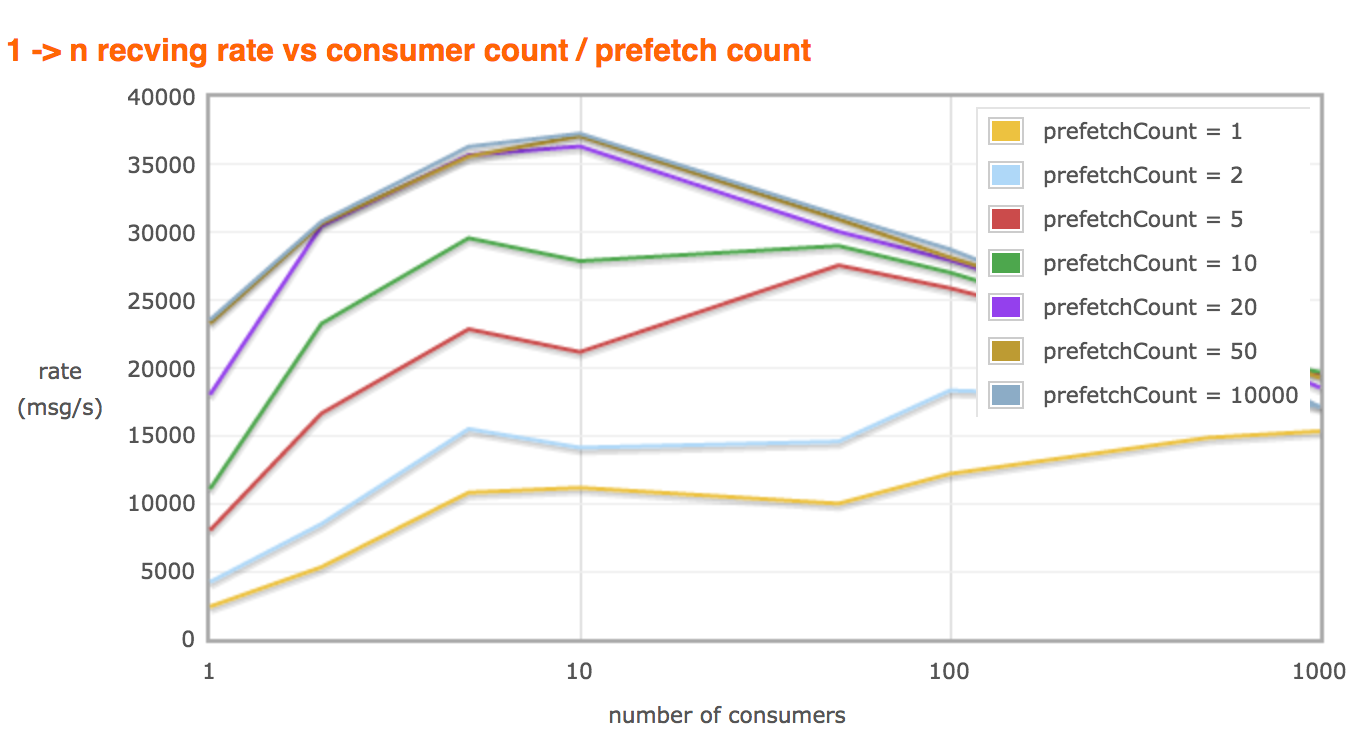
\includegraphics[width=1\textwidth]{figures/rabbitmqPrefetch}
  \caption[rabbitPerformance]{Chart showing performance variation when prefetch count is changed in the consumer\footnotemark}
\end{figure}
\footnotetext{\fullcite{rabbitmqPerformance}}

\section{STOMP}
\label{sec:stomp}
STOMP is the Simple (or Streaming) Text Orientated Messaging Protocol.
STOMP provides an interoperable wire format so that STOMP clients can communicate with any STOMP message broker to provide easy and widespread messaging interoperability among many languages, platforms and brokers. ~\parencite{stomp}
STOMP is a simple interoperable protocol designed for asynchronous message passing between clients via mediating servers. It defines a text based wire-format for messages passed between these clients and servers.
It is an alternative to other open messaging protocols such as AMQP and implementation specific wire protocols used in JMS brokers such as OpenWire. It distinguishes itself by covering a small subset of commonly used messaging operations rather than providing a comprehensive messaging API.
The main philosophies driving the design of STOMP are simplicity and interoperability.
STOMP is designed to be a lightweight protocol that is easy to implement both on the client and server side in a wide range of languages. This implies, in particular, that there are not many constraints on the architecture of servers and many features such as destination naming and reliability semantics are implementation specific.
  \subsection{Protocol Overview}
STOMP is a frame based protocol, with frames modeled on HTTP. A frame consists of a command, a set of optional headers and an optional body. STOMP is text based but also allows for the transmission of binary messages. The default encoding for STOMP is UTF-8, but it supports the specification of alternative encodings for message bodies.
A STOMP server is modeled as a set of destinations to which messages can be sent. The STOMP protocol treats destinations as opaque string and their syntax is server implementation specific. Additionally STOMP does not define what the delivery semantics of destinations should be. The delivery, or “message exchange”, semantics of destinations can vary from server to server and even from destination to destination. This allows servers to be creative with the semantics that they can support with STOMP.
STOMP does not, however, deal in queues and topics—it uses a SEND semantic with a “destination” string. The broker must map onto something that it understands internally such as a topic, queue, or exchange. Consumers then SUBSCRIBE to those destinations. Since those destinations are not mandated in the specification, different brokers may support different flavors of destination. So, it’s not always straightforward to port code between brokers. \cite{andyPiperVmware}

A STOMP client is a user-agent which can act in two (possibly simultaneous) modes:
\begin{itemize}
  \item as a producer, sending messages to a destination on the server via a SEND frame
  \item as a consumer, sending a SUBSCRIBE frame for a given destination and receiving messages from the server as MESSAGE frames.
\end{itemize}

  \subsection{STOMP Library for Dart}
  Given that dart is fairly new language, it does not yet have AMPQ client that can be used with RabbitMQ. As mentioned above in section~\ref{sec:rabbitmq} RabbitMQ also supports STOMP Protocol. An open source STOMP client in dart is available which was created by ‘Potix corporation’. It can perform most of the basic with a message broker system like connecting, creating queue, subscribing, enqueuing as well as dequeuing. Although it has those basic functionalities, it still has some limitations and incompleteness like lack of support of ‘Heartbeat’, only support STOMP version 1.2 or above.

\section{WebSockets}
The WebSocket Protocol enables two-way communication between a client running untrusted code in a controlled environment to a remote host that has opted-in to communications from that code.  The security model used for this is the origin-based security model commonly used by web browsers.  The protocol consists of an opening handshake followed by basic message framing, layered over TCP. The goal of this technology is to provide a mechanism for browser-based applications that need two-way communication with servers that does not rely on opening multiple HTTP connections (e.g., using XMLHttpRequest or <iframe>s and long polling).~\parencite{rfc6455}
The WebSocket Protocol provides a single TCP connection for traffic in both directions. Combined with the WebSocket API [WSAPI], it provides an alternative to HTTP polling for two-way communication from a web page to a remote server. It can be used for variety of web applications: games, stock tickers, multiuser applications with simultaneous editing, user interfaces exposing server-side services in real time, etc.

The WebSocket Protocol is designed to supersede existing bidirectional communication technologies that use HTTP as a transport layer to benefit from existing infrastructure (proxies, filtering, authentication). Such technologies were implemented as trade-offs between efficiency and reliability because HTTP was not initially meant to be used for bidirectional communication.

\subsection{Security}
The WebSocket Protocol uses the origin model used by web browsers to
restrict which web pages can contact a WebSocket server when the
WebSocket Protocol is used from a web page.  Naturally, when the
WebSocket Protocol is used by a dedicated client directly (i.e., not
from a web page through a web browser), the origin model is not
useful, as the client can provide any arbitrary origin string.
It is similarly intended to fail to establish a connection when data
from other protocols, especially HTTP, is sent to a WebSocket server,
for example, as might happen if an HTML "form" were submitted to a
WebSocket server.  This is primarily achieved by requiring that the
server prove that it read the handshake, which it can only do if the
handshake contains the appropriate parts, which can only be sent by a
WebSocket client.  In particular, at the time of writing of this
specification, fields starting with |Sec-| cannot be set by an
attacker from a web browser using only HTML and JavaScript APIs such
as XMLHttpRequest [XMLHttpRequest].

\subsection{Establishing a Connection}
When a connection is to be made to a port that is shared by an HTTP
server (a situation that is quite likely to occur with traffic to
ports 80 and 443), the connection will appear to the HTTP server to
be a regular GET request with an Upgrade offer.  In relatively simple
setups with just one IP address and a single server for all traffic
to a single hostname, this might allow a practical way for systems
based on the WebSocket Protocol to be deployed.  In more elaborate
setups (e.g., with load balancers and multiple servers), a dedicated
set of hosts for WebSocket connections separate from the HTTP servers
is probably easier to manage.  At the time of writing of this
specification, it should be noted that connections on ports 80 and
443 have significantly different success rates, with connections on
port 443 being significantly more likely to succeed, though this may
change with time.

\subsection{WebSocket URIs}
This specification defines two URI schemes, using the ABNF syntax
defined in RFC 5234 [RFC5234], and terminology and ABNF productions
defined by the URI specification RFC 3986 [RFC3986].
\newline
ws-URI = "ws:" "//" host [ ":" port ] path [ "?" query ]\newline
wss-URI = "wss:" "//" host [ ":" port ] path [ "?" query ]\newline
\newline
host = <host, defined in [RFC3986], Section 3.2.2>\newline
port = <port, defined in [RFC3986], Section 3.2.3>\newline
path = <path-abempty, defined in [RFC3986], Section 3.3>\newline
query = <query, defined in [RFC3986], Section 3.4>\newline

The port component is OPTIONAL; the default for "ws" is port 80,
while the default for "wss" is port 443.

The URI is called "secure" (and it is said that "the secure flag is
set") if the scheme component matches "wss" case-insensitively.

The "resource-name" (also known as /resource name/ in Section 4.1)
can be constructed by concatenating the following
\begin{itemize}
\item "/" if the path component is empty
\item the path component
\item "?" if the query component is non-empty
\item the query component
\end{itemize}

\section{RESTful WebServices}
